\documentclass{article}

\usepackage[spanish]{babel}

\usepackage[margin=1.5cm]{geometry}

\usepackage{arev}

\usepackage{hyperref}

\usepackage{subcaption}

\usepackage{amsmath}

\usepackage[style=alphabetic]{biblatex}
\addbibresource{refs.bib}

\usepackage{graphicx}
\graphicspath{{./imgs/}}

\usepackage{verbatimbox}

\usepackage{longtable}

\usepackage{tikz}

\newcommand{\furl}[1]{\footnote{\url{#1}}}

\title{
  Modelación y simulación computacional basada en agente\\
  Práctica 2: Modelos Basados en Agentes
}

\author{Edgar Quiroz}

\begin{document}
\maketitle

\begin{abstract}
  Se presenta la implementación, análsis y extensión de varios modelos de
  simulación basados en agentes.

  Entre ellos el modelo de segregación de Shelling\cite{Schelling_1971}, las
  termitas apiladores de Resnick\cite{10.5555/184223}, las hormigas caóticas de
  Miramontes\cite{Miramontes_1995} y el Loop de
  Langton\cite{langton84_self_reprod_cellul_autom}.

  Además, se propone como proyecto final implementar el modelo de colonia de
  hormigas \cite{Dorigo_1996} para resolver algún problema $NP$-Completo, por
  ejemplo el problema de encontrar la solución óptima a un cubo de Rubik
  \cite{Demaine_2018}.
\end{abstract}

\section{Generalidades}

Se realizaron las implementaciones usando \textit{mesa}
\furl{https://mesa.readthedocs.io}, una biblioteca de
Python para \textit{MBA}.

Ésta provee código reutilizable para definir agentes y entornos, además de de
visualización en vivo del modelo y múltiples herramientas para analizar
múltiples ejecuciones variando parmátros de entorno.

Junto con esas herramientos, se utilizó \textit{jupyter}
\furl{https://jupyter.org/}, \textit{pandas} \furl{https://pandas.pydata.org/} y
\textit{bokeh} \furl{https://bokeh.org/} para manipular y visualizar los
resultados.


\section{Segregación de Schelling}

El modelo propuesto originalmente por Thomas Schelling consiste en dos grupos
de agentes, por ejemplo, rojos y verdes, que localmente tratan de satisfacer la
necesidad de estar con los de su mismo grupo. De manera general este
comportamiento es establecido con un parámetro conocido como porcentaje de
similitud requerida o nivel de tolerancia.

Los agentes toman una decisión a partir de la información que tienen en su
vecindad. Si el agente satisface las condiciones del entorno entonces se queda
en su posición actual, de lo contrario, se mueve a una posición vacía.

Esta dinámica local genera como resultado la formación de cúmulos de agentes del
mismo tipo, es decir, hay segregación.

\subsection{Entorno}

El sistema se compone de una retícula de $n \times n$ donde $n$ se establece
usualmente entre 50 y 100. Cada celda con posición $(i,j)$ alberga a un agente
rojo o verde.
El sistema tiene un parámetro de densidad poblacional, usualmente se establece
en 0.9. La mitad de la población se inicializa como rojos y la otra como verdes.
Cada agente toma una celda de manera aleatoria.

\subsection{Dinámica}
Cada agente en la posición $(i,j)$ se “muda” a un lugar vacío si en su vecindad
de Moore (8-vecinos) no cumple con el porcentaje de similitud requerida.

\subsection{Actividades}

\subsubsection{Implementación}

Implemente el modelo de segregación de Schelling original \cite{Schelling_1971}.
Puntos extra si no es en \textit{NetLogo}.

Se realizó la implementación en \textit{python} usando el módulo de
\textit{mesa}. La interfaz resultante se puede ver en \ref{fig:sch-ui}.

\begin{figure}
  \centering
  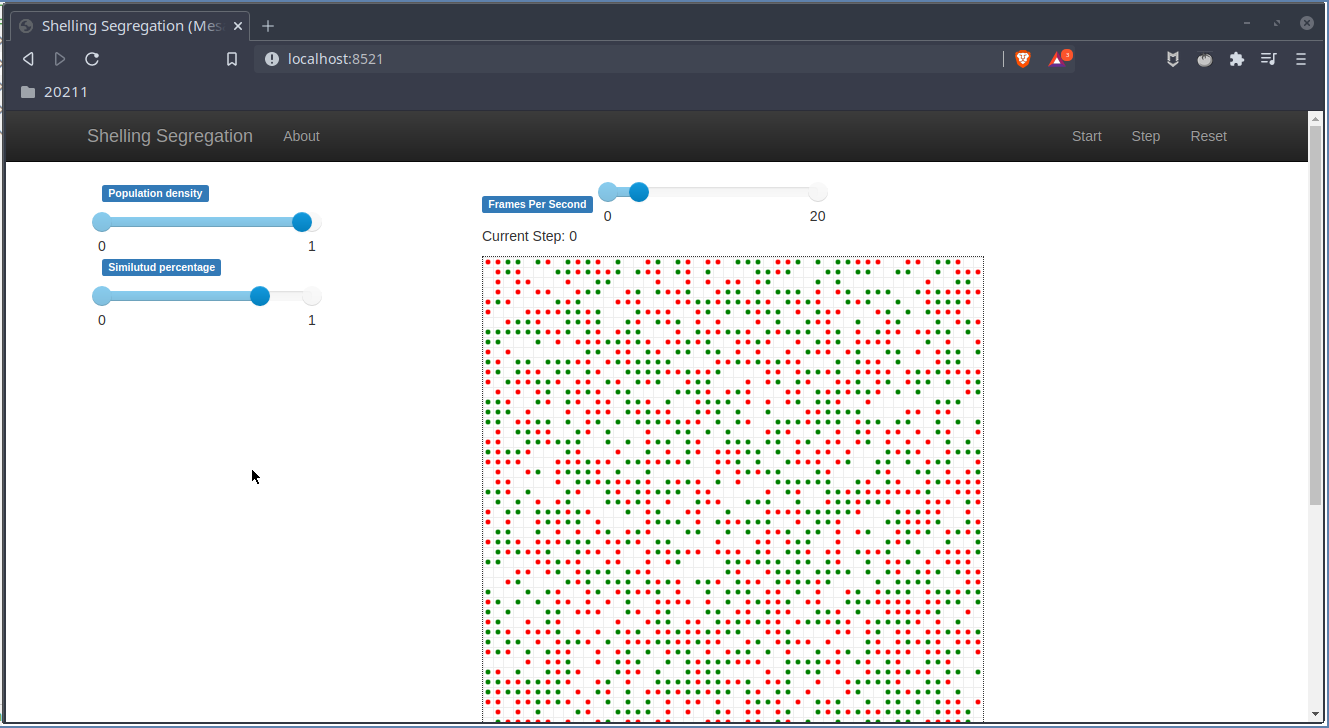
\includegraphics[width=0.9\textwidth]{imgs/shelling-ui.png}
  \caption{Interfaz gráfica del modelo de segregación de Schelling}
  \label{fig:sch-ui}
\end{figure}

\subsubsection{Límite de similitud}

Establezca el tamaño de la retícula como $n = 50$, con densidad de población
$0.9$.
¿Qué valor del parámetro de similitud es el límite máximo para formar dinámicas
de segregación?
A este valor le llamaremos $S_{max}$.

Determinar si hay una segregación puede ser bastante complicado, pues habría que
definir un método estadísitico para medirla. Aún así, si es sufientemente
fuerte, se puede apreciar a simple vista.

En la figura \ref{fig:sim-max} se pueden ver dos ejecuciones del modelo. La
variación de la similitud es muy pequeña pero el cambio en la dinámica es
notable. Si bien en la figura \ref{fig:sim755} se podría argumentar que hay
inicios de cúmulos, el hecho de que no se haya formado nada aún después de 500
pasos significa que no hay tendencia a formar cúmulos significativos.

Así que a grandes rasgos, $S_{max} \approx 0.75$ con los parámetros dados.

\begin{figure}
  \centering
  \begin{subfigure}{0.4\textwidth}
    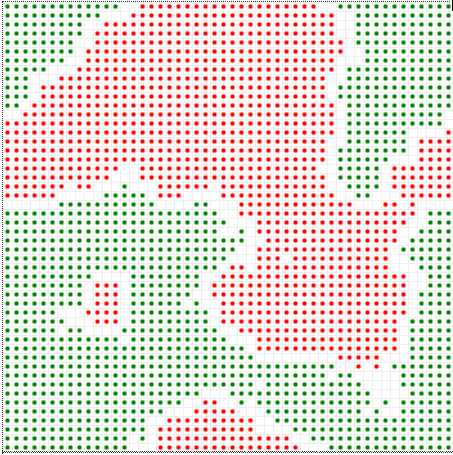
\includegraphics[width=\textwidth]{imgs/conv_state75.png}
    \caption{$sim=0.75$ después de 120 pasos}
    \label{fig:sim75}
  \end{subfigure}
  \quad
  \begin{subfigure}{0.4\textwidth}
    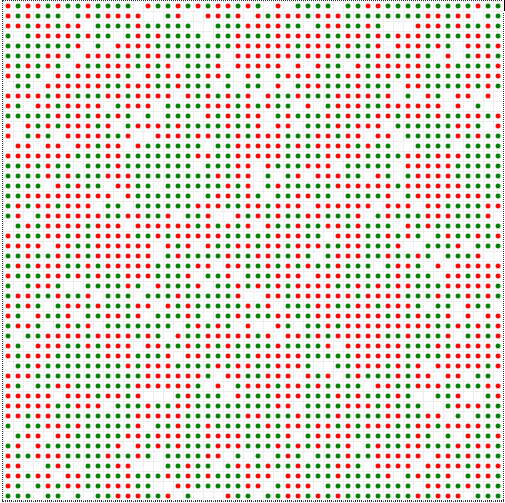
\includegraphics[width=\textwidth]{imgs/sim755.png}
    \caption{$sim=0.755$ después de 500 pasos}
    \label{fig:sim755}
  \end{subfigure}
  \caption{Estimación de $S_{max}$}
  \label{fig:sim-max}
\end{figure}

\subsubsection{Límite de convergencia}

Una propuesta de medida para detectar convergencias es cuando los agentes ya no
cambian de posición.

\begin{itemize}
  \item Cuándo el parámetro de similitud es igual a $S_{max}$, ¿cuál es el
    tiempo en el que el sistema converge?

    En la figura \ref{fig:conv75} se tiene una ejecución convergente con
    $sim = S_{max} = 0.75$. Se puede ver como en la configuracón en
    \ref{fig:state-conv75} hay una frontera muy marcada entre los dos grupos. Y
    al final de la gráfica en \ref{fig:chart-conv75} la cantidad de agentes
    satisfechos se estabiliza al rededor de 2250.

    \begin{figure}
    \centering
    \begin{subfigure}{0.4 \textwidth}
        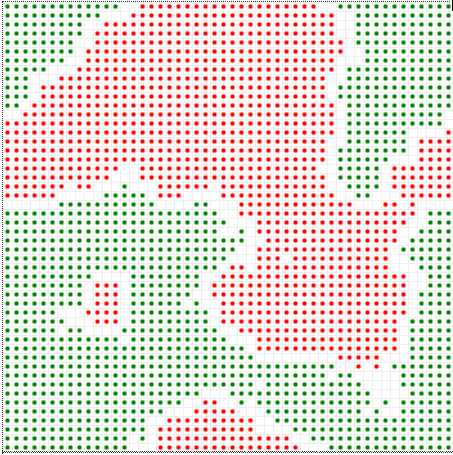
\includegraphics[width=\textwidth]{imgs/conv_state75.png}
        \caption{Configuración estable con $sim = S_{max}$}
        \label{fig:state-conv75}
    \end{subfigure}
    \quad
    \begin{subfigure}{0.5\textwidth}
        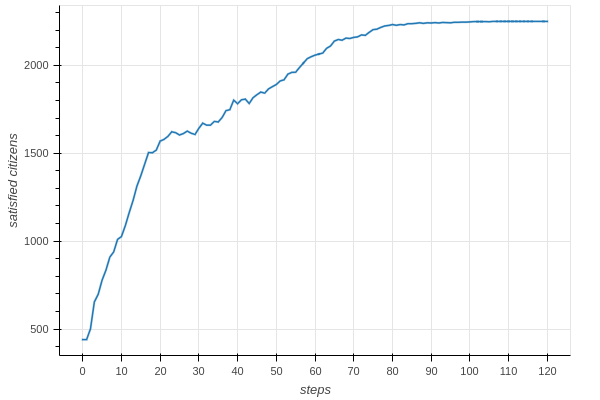
\includegraphics[width=\textwidth]{imgs/conv_chart75.png}
        \caption{Satisfacción con $sim = S_{max}$}
        \label{fig:chart-conv75}
    \end{subfigure}
    \caption{Convergencia con $sim=S_{max}$}
    \label{fig:conv75}
    \end{figure}

  \item Forme una gráfica de similitud contra tiempo de convergencia. ¿Cómo
    crece/decrece el tiempo de convergencia ? ¿lineal, logarítmico, exponencial?

    Un agente se mueve si y sólo si no está satisfecho, así que se considera
    esta cantidad en lugar de contar directamente si los agentes se mueve. Pero
    podría ser que un agente insatisfecho, al moverse, siga insatisfechos. Así
    que podría ser que la cantidad de agentes satisfechos no cambie aunque sí
    haya movimiento.

    Una manera de prevenir esto es esperar a que la cantidad de agentes
    satisfechos no cambie por varios turnos. Entre más turnos, menor la
    posibilidad de que haya movimiento a pesar de que la cantidad no cambie.
    En este caso, se esperó a que la cantidad se mantuviera constante por diez
    pasos.

    Para valores de similitud mayores a $S_{max}$, el sistema no va a converger.
    Así que solo se probaron valores en $0-0.75$, con 400 pasos como máximo. La
    gráfica resultante está en la figura \ref{fig:conv-sim}.

    \begin{figure}
    \centering
    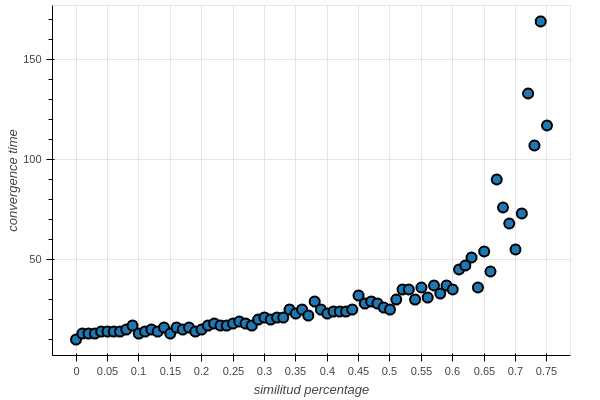
\includegraphics[width=0.75\textwidth]{imgs/sim_conv.png}
    \caption{Tiempo de convergencia}
    \label{fig:conv-sim}
    \end{figure}

    A simple vista, parece una función exponencial creciente.

\end{itemize}

\subsubsection{Similitud normal}

Establezca el parámetro de similitud como un atributo de los agentes. Inicialice
la similitud requerida del agente $i$-ésimo a partir de una distribución normal.

\begin{itemize}
  \item Con media 50 y desviación estándar 10.¿Cómo cambian los patrones de
    segregación?

    El sistema converge estrictamente en aproximadamente 100 iteraciones, pero
    si se observa la figura, desde la iteración 20 se tiene un valor muy
    estable. Para comparar, con desviación estándar 0, el sistema converge
    estrictamente en 20 iteraciones.

    Este se puede deber a que una media de 50 es bastante tolerable, y la
    desviación es lo suficientemente pequeña para que el sistema se comporte
    casicomo si no hubiera desviación estándar.

    La convergencia con desviación 0 y 10 se puede ver en la figura
    \ref{fig:sche-n50}

    \begin{figure}
      \centering
      \begin{subfigure}{0.4\textwidth}
        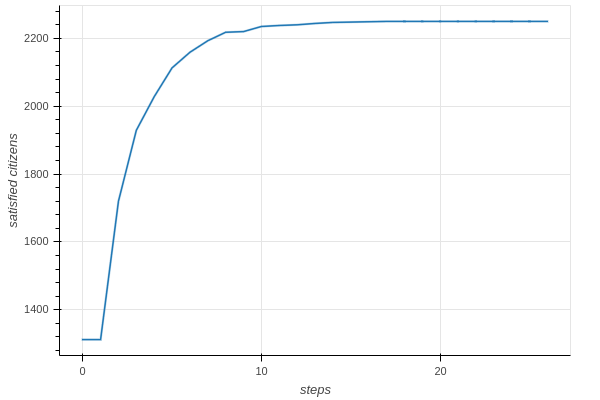
\includegraphics[width=\textwidth]{imgs/const50.png}
        \caption{Convergencia con media 50 y desviación estándar 0}
        \label{fig:sche-n500}
      \end{subfigure}
      \quad
      \begin{subfigure}{0.4\textwidth}
        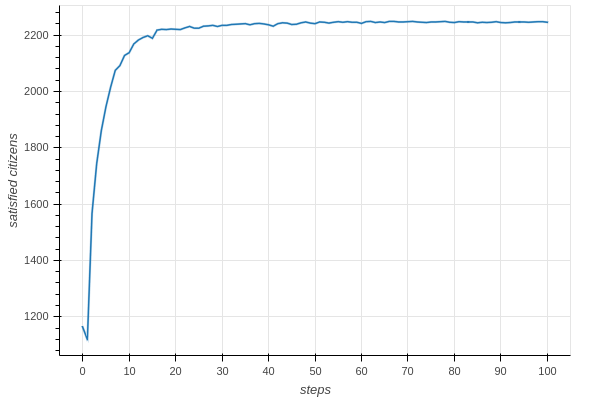
\includegraphics[width=\textwidth]{imgs/normal50.png}
        \caption{Convergencia con media 50 y desviación 10}
        \label{fig:sche-n5010}
      \end{subfigure}
      \caption{Convergencia con media 50}
      \label{fig:sche-n50}
    \end{figure}

  \item ¿Y con media = $S_{max}$ y desviación estándar pequeña y grande?

    La media cerca de $S_{max}$ hace el sistema increíblemente inestable, por lo
    que deja de converger inclusive con una mínima desivación, como se puede ver
    en la figura \ref{fig:sche-smax-min}. Con una gran desviación, los saltos
    son aún más erráticos, como se ve en la figura \ref{fig:sche-smax-max}.

    \begin{figure}
      \centering
      \begin{subfigure}{0.4\textwidth}
        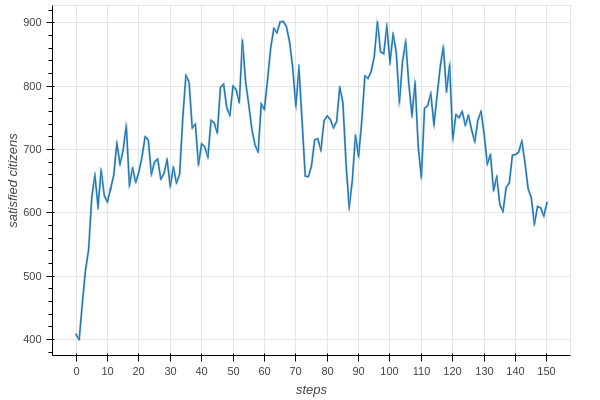
\includegraphics[width=\textwidth]{imgs/norm_smax_min.png}
        \caption{Convergencia con media $S_{max}$ y desviación estándar 0.0001}
        \label{fig:sche-smax-min}
      \end{subfigure}
      \quad
      \begin{subfigure}{0.4\textwidth}
        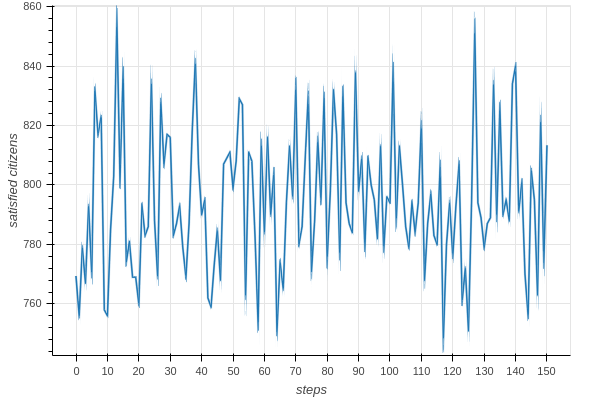
\includegraphics[width=\textwidth]{imgs/norm_smax_max.png}
        \caption{Convergencia con media 50 y desviación 50}
        \label{fig:sche-smax-max}
      \end{subfigure}
      \caption{Convergencia con media $S_{max}$}
      \label{fig:sche-n50}
    \end{figure}

\end{itemize}

\subsubsection{Maś grupos}

Modifique su programa previo para considerar tres tipos de agentes (rojos,
verdes y azules). Inicialice cada grupo como $\frac{1}{3}$ de la población y
establezca de manera global el parámetro de similitud requerida.

\begin{itemize}
  \item ¿Se forman patrones de segregación?

    Sí, se forman cúmulos similares, solo que separados en tres tipos en lugar
    de solo dos. Un ejemplo de una ejecución que ha convergido se puede ver en
    la figura \ref{fig:sche-conv3}.

    \begin{figure}
      \centering
      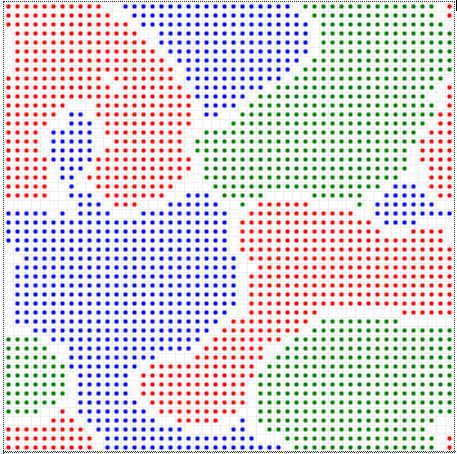
\includegraphics[width=0.4\textwidth]{imgs/3conv.png}
      \caption{Convergencia con tres grupos}
      \label{fig:sche-conv3}
    \end{figure}
  \item ¿Cuál es el valor de umbral de $S_{max}$?

    Por prueba y error, se encontró que al rededor de $0.625$ es el punto donde
    el sistema deja de converger. Para ilustrar esto, en la figura
    \ref{fig:sche-3smax} se puede ver como un paso de tan solo $0.001$ hace que
    el sistema ya no converga.

    \begin{figure}
      \centering
      \begin{subfigure}{0.4\textwidth}
        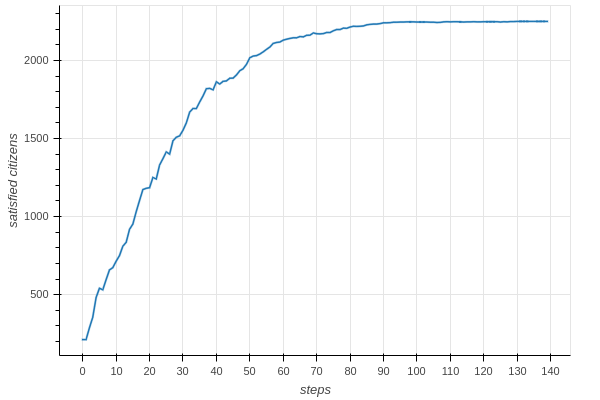
\includegraphics[width=\textwidth]{imgs/3_625.png}
        \caption{Convergencia con $sim=0.625$}
        \label{fig:sche-3-0625}
      \end{subfigure}
      \begin{subfigure}{0.4\textwidth}
        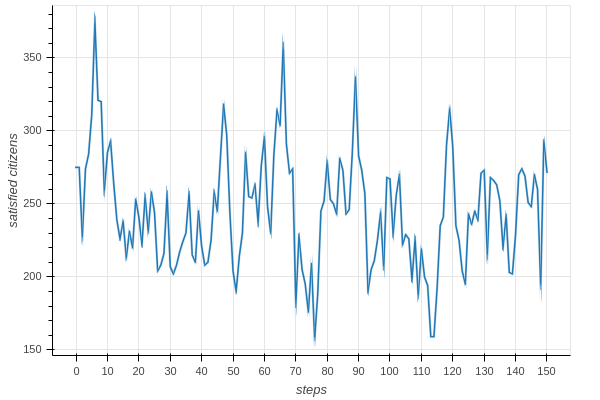
\includegraphics[width=\textwidth]{imgs/3_6251.png}
        \caption{Divergencia con $sim=0.6251$}
        \label{fig:sche-3-06251}
      \end{subfigure}
      \caption{$S_{max}$ con tres grupos}
      \label{fig:sche-3smax}
    \end{figure}
\end{itemize}


\subsubsection{Otras propuestas}

\begin{itemize}
  \item¿Qué otros elementos de modelación se podrían definir en el modelo de
    Schelling para hacerlo más realista?

    Se podría definir diferentes similitudes en función del grupo, simbolizando
    que algunos grupos pueden ser más tolerantes que otros.

    O también, se podría hacer que la similitud requerida cambie dependiendo de
    las interacciones son los otros agentes, haciéndola un valor dinámico.

  \item ¿Qué otro análisis se podría implementar para explicar las dinámicas?

    Se podrían calcular varios aspectos de los cúmulos, como su tamaño promedio,
    o su dimensión fracta de los cúmulos. Menor
    dimensión y mayor tamaño significaría grupos más uniformes y cerrados.
\end{itemize}

\section{Termitas apiladoras}

Este modelo fue propuesto por Mitchel Resnick \cite{10.5555/184223} como una
estrategia decentralizada para apilar astillas de madera a través de simples
reglas ejecutadas por termitas.

\subsection{Entorno}

El sistema se compone de una retícula de $100 \times 100$. Al inciciar, se
colocan aleatoriamente $n$ termintas, y se colocan astillas es una fracción $d$
de la retícula.

\subsection{Dinámica}

Las termitas tienen dos reglas básicas.

\begin{itemize}
  \item Si la termita no está cargando nada y se encuentra una astilla, la
    recoge
  \item Si está cargando una astilla y se encuentra otra, la suelta y sigue su
    camino.
\end{itemize}

Las termitas realizan una caminata aleatoria con apertura de visión de $-50$ a
$50$ grados.

\subsection{Actividades}

\subsubsection{Implementación}

Implemente el modelo de termitas apiladoras. Punto extra si no es en
\textit{NetLogo}.

Se realizó la implementación con \textit{mesa}. La visuaización resultante se
puede ver en la figura \ref{fig:termite-ui}.

\begin{figure}
  \centering
  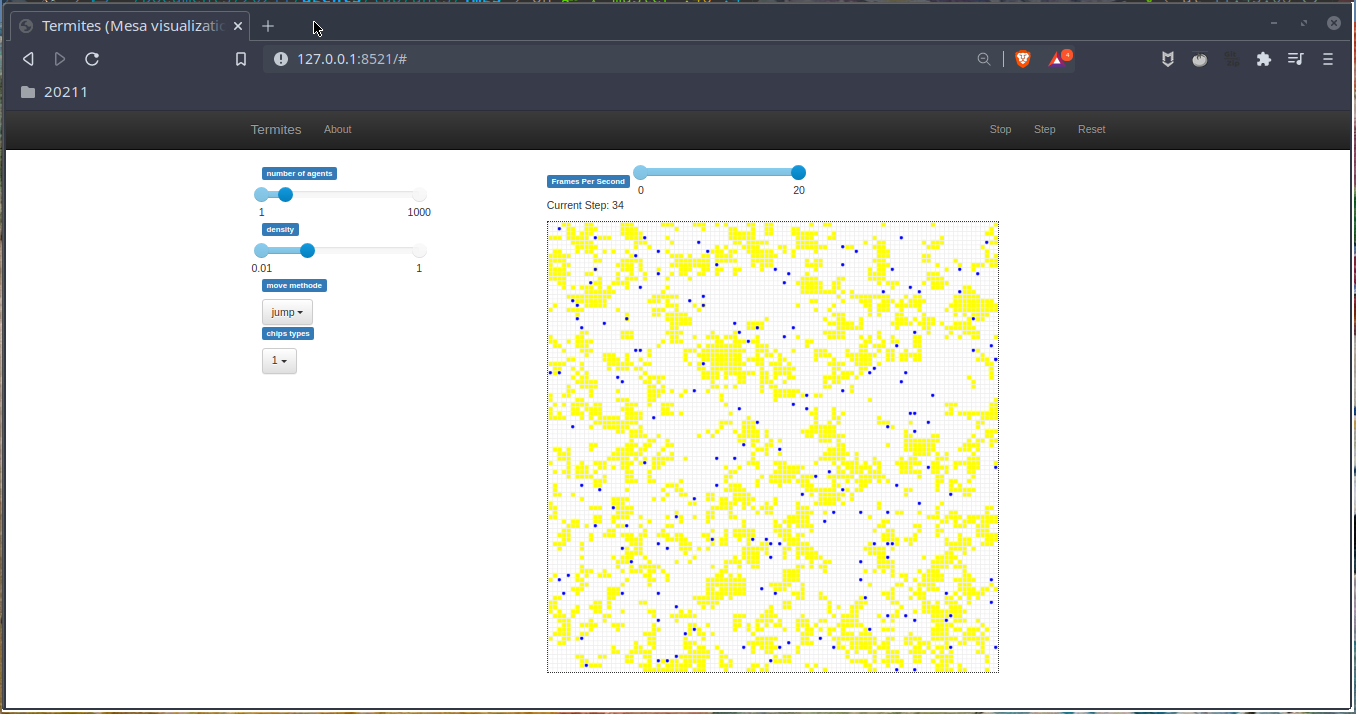
\includegraphics[width=0.9\textwidth]{imgs/termites-ui.png}
  \caption{Interfaz gráfica del modelo de termitas}
  \label{fig:termite-ui}
\end{figure}

\subsubsection{Recolección de datos}

Implemente la recolección de varios datos del sistema al progresar el tiempo. En
particular, el número de cúmulos, el tamaño promedio de los cúmulos, y el número
de termitas cargando astillas. Argumente porque cada medida es útil para
entender el sistema.

\subsubsection{Más tipo de astillas}

Extienda el modelo considerando dos tipos de astillas (amarillas y cafés). Las
termintas solo sueltan las astillas al encontrar otra del mismo color. ¿Cuántos
cúmulos quedan al final? Muestre la visualización de la evolución del sistema.

\begin{figure}
  \centering
  \begin{subfigure}{0.3\textwidth}
    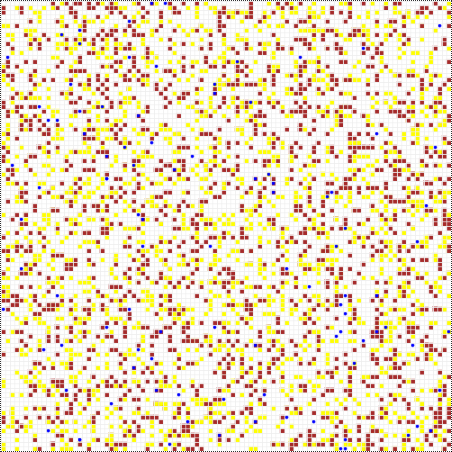
\includegraphics[width=\textwidth]{imgs/termites-chips1.png}
    \caption{0 pasos}
  \end{subfigure}
  \begin{subfigure}{0.3\textwidth}
    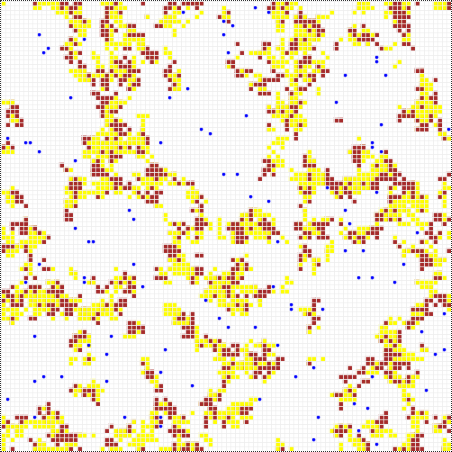
\includegraphics[width=\textwidth]{imgs/termites-chips3.png}
    \caption{100 pasos}
  \end{subfigure}
  \begin{subfigure}{0.3\textwidth}
    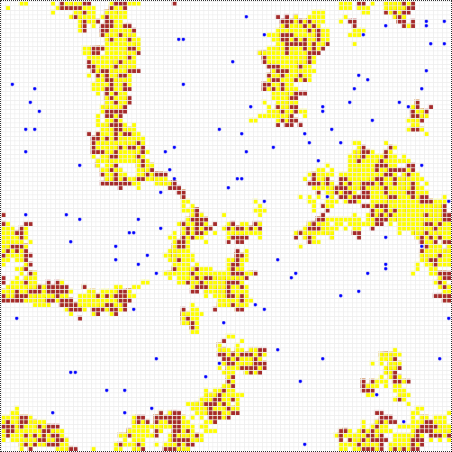
\includegraphics[width=\textwidth]{imgs/termites-chips5.png}
    \caption{200 pasos}
  \end{subfigure}
  \caption{Evolución con dos tipos de astilla}
  \label{fig:termite-2chips}
\end{figure}

Una ejecución de esta variante se puede ver en la figura
\ref{fig:termite-2chips}. No se forman cúmulos homogéneos. Las astilas de
diferente color se ``estorban'' entre sí, impidiendo que se formen cúmulos
grandes.

\subsubsection{Caminata con saltos}

En la regla original, al soltar la astilla se sigue el camino normal. En lugar
de eso, haga que la termita salte a otra posición de manera aleatoria. ¿Cómo
cambian los patrones formados? Muestre la visualización de la evolución del
sistema y explique su comportamiento. ¿Esto se deduce a partir de las reglas
locales?

\begin{figure}
  \centering
  \begin{subfigure}{0.3\textwidth}
    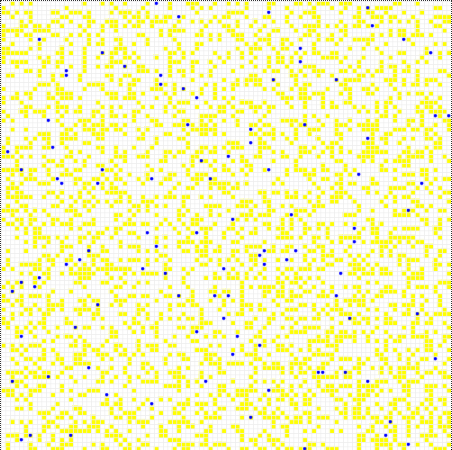
\includegraphics[width=\textwidth]{imgs/termites-teleport1.png}
    \caption{0 pasos}
  \end{subfigure}
  \begin{subfigure}{0.3\textwidth}
    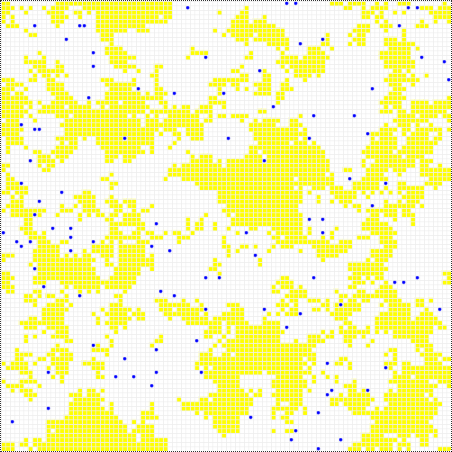
\includegraphics[width=\textwidth]{imgs/termites-teleport3.png}
    \caption{100 pasos}
  \end{subfigure}
  \begin{subfigure}{0.3\textwidth}
    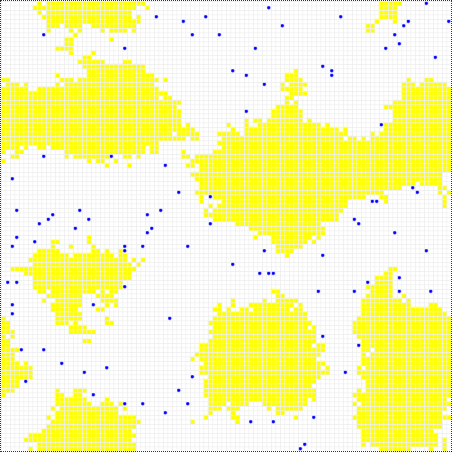
\includegraphics[width=\textwidth]{imgs/termites-teleport5.png}
    \caption{200 pasos}
  \end{subfigure}
  \caption{Evolución de termitas con saltos}
  \label{fig:termite-teleport}
\end{figure}

Una ejecución de esta variantes se puede ver en la figura
\ref{fig:termite-teleport}. Inicialmente se forman ``franjas'' de astillas en
lugar de cúmulos, aunque eventualmente se converge a cúmulos. Una explicación es
que originalmente, una termite evita adentrarse en los cúmulos. Esto genera una
barrea de cúmulos que normalmente no pueden pasar, así que las termitas suelen
quedarse es una misma área, lo que hace más grandes los cúmulos existentes en
esa área. Pero con el salto aleatorio, pueden viajar a cualquier parte del
tablero, tomando y quitando de todos los cúmulos por igual, lo que provoca estas
delgadas franjas.

Esto es un comportamiento emergente, que no se habría podido deducir de las
reglas sin realizar algún tipo de simulación.

\section{Hormigas al borde del caos}

Las hormigas \textit{Leptothorax} son una especia caracterizada
por sus colonias pequeñas, de veinte a cien individuos, la carencia de reinas y
sus patrones aparentemente aleatorios entre trabajar y descansar para alguna
hormiga. Aún así, a nivel de colonial presentan gran coordinación y eficacia.

Usando información de estudios biológicos, Miramontes \cite{Miramontes_1995}
propuso un modelo para simular los periodos de trabajo reposo en colonias de
hormigas artificiales. En este, se colocan hormigas artificales en una fracción
$d$ de una malla. Con una $d$ pequeña, las hormigas no interactuan y todo su
comportamiento es aleatorio. Con una $d$ grande, las hormigas se sincronizan,
trabajando y descansando exactamente en los mismo periodos.

Los experimentos mostraron que las colonias reales tienen una densidad en un
punto intermedio, donde las hormigas interatúan y se sincronizan, pero aún
tienen libertad suficiente para realizar acciones aleatorias. Están al borde del
caos.

\subsection{Entorno}

La colonia está representada por una malla de $10 \times 10$. Cada casilla puede
estar vacía o contener una hormiga. Al inicia, se colocan hormigas aleatoramente
en una fracción $d$ de la malla.

\subsection{Dinámica}

Cada hormiga puede estar activada o no. Puede pasar de inactiva a activa de dos
formas. Primero, con una probabilidad $p_{a}$ de forma expontánea. Luego, cuando
otra hormiga activa entre a vecindad de Moore.

Una vez activa, una hormiga se mueve de manera aleatoria, una casilla a la vez.
Al activarse, una hormiga adquiere una energía inicial $s_{a}$. A partir de ese
momento, su energía evoluciona de la siguiente manera

\begin{equation}
  s_{i}(t) = \tanh(g \cdot ((\sum_{j \in N(i)}{s_{i}(t-1)}) + s_{i}(t-1))
\end{equation}

donde $g$ es una constante llamada ganancia y $N(i)$ es la vecindad de Moore de
$i$. Al llegar la energía a un valor menor a $\varepsilon$, se considera que la
energía es cero, y la hormiga se desactiva. Siguiendo los experimentos de
Miramontes, se toma $\varepsilon = 10^{-16}$, $s_{a} = 10^{-6}$ ,
$p_{a} = 10^{-2}$ y $0.005 \le g \le 0.5$.


\subsection{Actividades}

\subsubsection{Implementación}

Implemente un modelo basdo en agentes donde considere las siguientes
caracterísiticas

\begin{itemize}
  \item La función de activación (tangente hiperbólica)
  \item La vecinad de Moore
  \item El movimiento aleatorio de las hormigas
  \item El tamaño de la retícula
  \item El tamaño de la población
\end{itemize}

Como todas las implementaciones, se usó \textit{mesa} para hacer la simulación.
La visualización resultante se puede ver en la figura \ref{fig:ant-ui}.

\begin{figure}
  \centering
  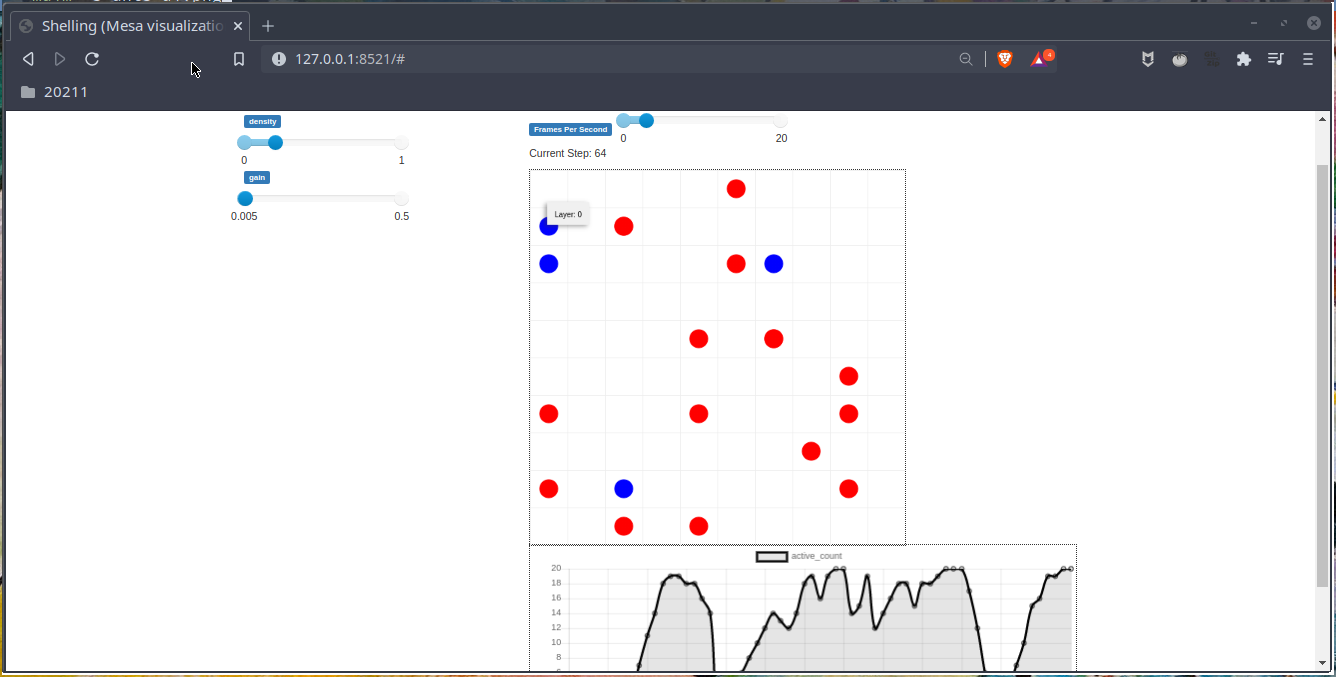
\includegraphics[width=\textwidth]{imgs/ants-ui.png}
  \caption{Interfaz gráfica de las hormigas caóticas}
  \label{fig:ant-ui}
\end{figure}

\subsubsection{Series de tiempos de activación}

Cree las series de tiempo de activación para distintas densidades de a población
de hormigas. Específicamente, contar las hormigas que se encuentran en estado
activo en el tiempo $t$, y grafica la evolución durante 600 tiempos.

Se realizaron ejecuciones con densiad de 0.01, 0.1, 0.2, 0.3, 0.5 y 0.9. En la
figura \ref{fig:ds} se puede ver dichas series.

\begin{figure}
  \centering
  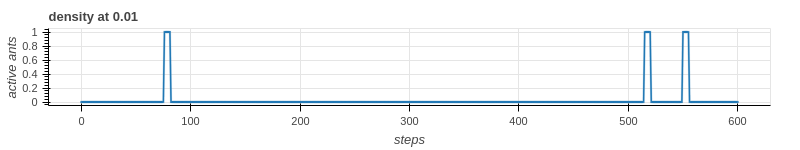
\includegraphics[width=\textwidth]{imgs/ant001.png}
  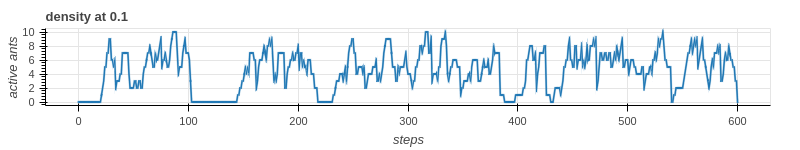
\includegraphics[width=\textwidth]{imgs/ant01.png}
  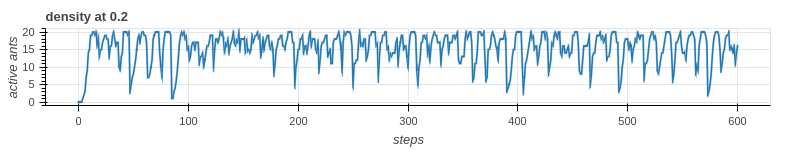
\includegraphics[width=\textwidth]{imgs/ant02.png}
  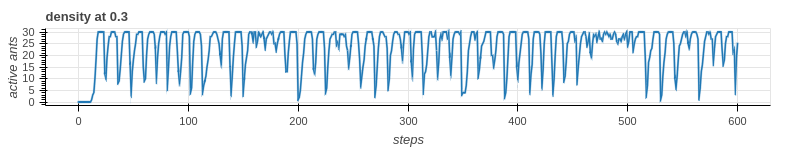
\includegraphics[width=\textwidth]{imgs/ant03.png}
  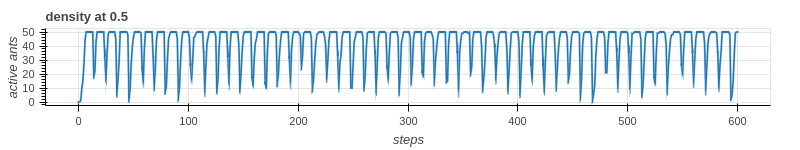
\includegraphics[width=\textwidth]{imgs/ant05.png}
  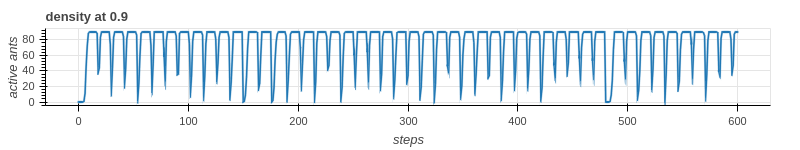
\includegraphics[width=\textwidth]{imgs/ant09.png}
  \caption{Series de tiempo con varias densiades}
  \label{fig:ds}
\end{figure}

\subsubsection{Transición orden/desorden}

Mostrar con varias series de tiempo que al rededor de $d=0.2$ el sistema exhibe
una transición de fase. Explicar a detalle.

En la figura \ref{fig:ant-chaos} se tienen las series de tiempo para valores de
$d$ alrededor de $0.1$, cuando la series es caótica, y $0.3$, donde la serie es
prácticamente periódica.

A partir de $1.5$, se puede ver que empiezan a surgir secciones sincronizadas,
entre los tiempos 75 y 125, o entre 250 y 300. Análogamente, en $0.25$ aún hay
periodos caóticos, como entre 400 y 450.

En $0.2$ no hay nada claro. A grandes rasgos toda la serie es periódica, pero
los cambios entre periodos no son tan marcados, y dentro de cada uno aún hay
secciones caóticas no tan marcadas.

Como explica Miramontes, esto puede ser debido a que en $d=0.1$, por ejemplo,
las hormigas están lo suficientemente dispersadas para ignorarse entre sí. Esto
resulta en únicamente activaciones aleatorias. Por otro lado, en $d=0.3$, hay
tantas hormigas que no se pueden dar espacio entre sí. Así que al activarse
una, todas se activan, su energía disminuye maś o menos al mismo ritmo, por lo
que las secciones de reposo también se sincronizan. En $d=0.2$, hay una una
cantidad de hormigas tal que pueden interatuar constantemente, pero dándonse
suficiente espacio para poder tomar decisiones individuales sin afectar
directamente al resto de las hormigas.

\begin{figure}
  \centering
  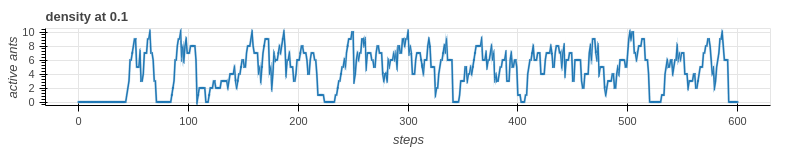
\includegraphics[width=\textwidth]{imgs/chaos01.png}
  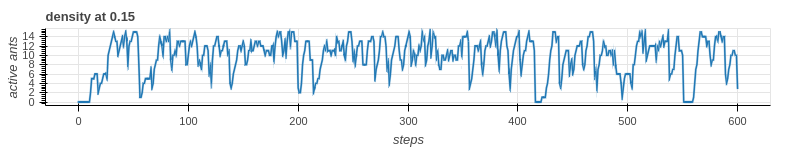
\includegraphics[width=\textwidth]{imgs/chaos015.png}
  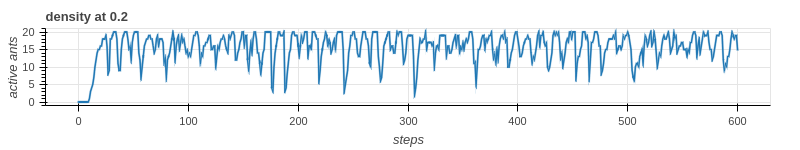
\includegraphics[width=\textwidth]{imgs/chaos02.png}
  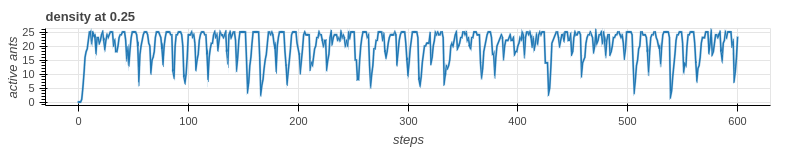
\includegraphics[width=\textwidth]{imgs/chaos025.png}
  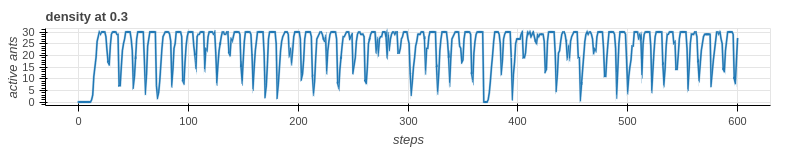
\includegraphics[width=\textwidth]{imgs/chaos03.png}
  \caption{Series de tiempo al rededor de $d=0.2$}
  \label{fig:ant-chaos}
\end{figure}

\subsubsection{Compresión}

Usar algún algoritmo de compresión (tar, gzip, bzi, tgz, rar, etc.) para
compactar algunas de las series de tiempo. Medir la tasa de compresión para cada
una de las series, variando densidades entre $0.01$ y $1$. Graficar los
resultados.

Se computaron dos series de tiempo para cada valor de densidad entre 0 y 1 con
un paso $0.01$. Luego, se extrajeron los valores y se pusieron en una cadena,
separados por espacios. Estas cadenas se comprimieron usando el módulo
\textit{zlib}\furl{https://www.zlib.net/} de \textit{python}, una implementación
método LZ77, el mismo usado en \textit{gzip}.

Todas las series de tiempo tienen una longitud de 600, así que la tasa de
compresión se tomó como la longitud de la cadena comprimida.

Los valores resultantes se pueden ver en la figura \ref{fig:ant-compress}. Se
puede ver un máximo aproximadamente en $d=0.2$, que corresponde al borde del
caos y orden observado en las series visualizadas.

\begin{figure}
  \centering
  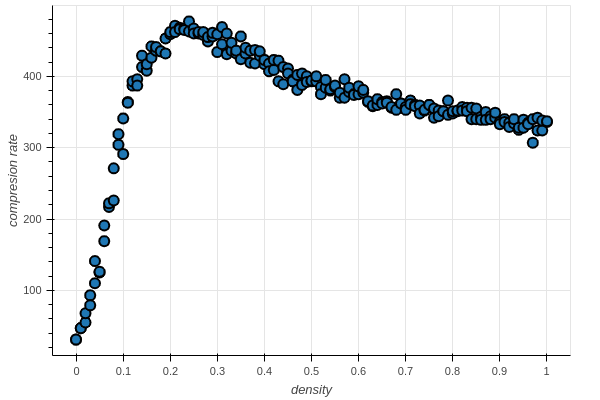
\includegraphics[width=0.75\textwidth]{imgs/compression.png}
  \caption{Tasa de compresión en función de densidad}
  \label{fig:ant-compress}
\end{figure}

\section{Loop de Langton}

Christopher Langton mostró la capacidad de autoreproducción de los autómatas
celuladres a partir de los modelos de von Neuman y Codd
\cite{langton84_self_reprod_cellul_autom}. El loop de Langton es un modelo
simple que satisface los criterios de autoreproducción. Esta estrucutura logra
su simplicidad almacenando su descripción en un ``loop'' dinámico.

El modelo se desarrolla en un autómata celular bidimensional con ocho posibles
estados en sus celdas y considerando la vecindad de Neuman para las
transiciones.

\subsection{Estados}

\begin{itemize}
  \item El estado cero son celdas muertas o inactivas.
  \item Estado 1 representa el canal interno del loop.
  \item Estado 2 es la coraza que protege al canal.
  \item 4, 5, 6, y 7 (seguidos de un 0) son codificaciones de la información
    que viaja por los canales.
  \item El estado 3 indica a la apertura o cierre de canales.
\end{itemize}

Usando los estados recien definidos, la configuración inicial se puede ver en la
figura \ref{fig:langton-init}. Los espacios vacíos representan al estado 0.

\begin{verbbox}
  2 2 2 2 2 2 2 2
2 1 7   1 4   1 4 2
2   2 2 2 2 2 2   2
2 7 2         2 1 2
2 1 2         2 1 2
2   2         2 1 2
2 7 2         2 1 2
2 1 2 2 2 2 2 2 1 2 2 2 2 2
2 0 7 1 0 7 1 0 7 1 1 1 1 1 2
  2 2 2 2 2 2 2 2 2 2 2 2 2
\end{verbbox}

\begin{figure}
  \centering
  \theverbbox
  \caption{Configuración inicial del Loop de Langton}
  \label{fig:langton-init}
\end{figure}

\subsection{Transiciones}

Como se considera una vecindad de von Neuman, entonces la función de transición
debe tomar en cuenta los cuatros vecinos además de la celda acutual. Esto es
$f: S^{5}\to S$, con $S$ conjunto de estados. Esto da un total de $8^{5} =
32768$ entradas. Como son bastantes, Langton codificó varias de ellas. Primero,
todas las reglas son invariantes ante rotaciones de la vecindad.
Es decir, si $(a, b, c, d, e)$ es una entrada de la función, entonces a
$(a, c, d, e, b), (a, d, e, b, c)$ y $(a, e, b, c, d)$ les corresponde la misma
regla. Además, no se muetran las reglas inválidas.

Aún así, el compendio de reglas es bastante amplio. Se presenta en la tabla
\ref{tab:langton}. Hay que notar que el orden CTRBL $\to$ I corresponde a la
denominación de la figura \ref{fig:langton-nom}.

\begin{verbbox}
  T
L C R => I
  B
\end{verbbox}

\begin{figure}
  \centering
  \theverbbox
  \caption{Nomenclatura de las vecindades}
  \label{fig:langton-nom}
\end{figure}

\begin{table}
  \begin{longtable}{| c | c | c | c | c |}
    \hline
    CTRBL$\to$I & CTRBL$\to$I & CTRBL$\to$I & CTRBL$\to$I & CTRBL$\to$I\\
    \hline
    00000$\to$0 & 02527$\to$1 & 11322$\to$1 & 20242$\to$2 & 30102$\to$1\\
    00001$\to$2 & 10001$\to$1 & 12224$\to$4 & 20245$\to$2 & 30122$\to$0\\
    00002$\to$0 & 10006$\to$1 & 12227$\to$7 & 20252$\to$0 & 30251$\to$1\\
    00003$\to$0 & 10007$\to$7 & 12243$\to$4 & 20255$\to$2 & 40112$\to$0\\
    00005$\to$0 & 10011$\to$1 & 12254$\to$7 & 20262$\to$2 & 40122$\to$0\\
    00006$\to$3 & 10012$\to$1 & 12324$\to$4 & 20272$\to$2 & 40125$\to$0\\
    00007$\to$1 & 10021$\to$1 & 12327$\to$7 & 20312$\to$2 & 40212$\to$0\\
    00011$\to$2 & 10024$\to$4 & 12425$\to$5 & 20321$\to$6 & 40222$\to$1\\
    00012$\to$2 & 10027$\to$7 & 12426$\to$7 & 20322$\to$6 & 40232$\to$6\\
    00013$\to$2 & 10051$\to$1 & 12527$\to$5 & 20342$\to$2 & 40252$\to$0\\
    00021$\to$2 & 10101$\to$1 & 20001$\to$2 & 20422$\to$2 & 40322$\to$1\\
    00022$\to$0 & 10111$\to$1 & 20002$\to$2 & 20512$\to$2 & 50002$\to$2\\
    00023$\to$0 & 10124$\to$4 & 20004$\to$2 & 20521$\to$2 & 50021$\to$5\\
    00026$\to$2 & 10127$\to$7 & 20007$\to$1 & 20522$\to$2 & 50022$\to$5\\
    00027$\to$2 & 10202$\to$6 & 20012$\to$2 & 20552$\to$1 & 50023$\to$2\\
    00032$\to$0 & 10212$\to$1 & 20015$\to$2 & 20572$\to$5 & 50027$\to$2\\
    00052$\to$5 & 10221$\to$1 & 20021$\to$2 & 20622$\to$2 & 50052$\to$0\\
    00062$\to$2 & 10224$\to$4 & 20022$\to$2 & 20672$\to$2 & 50202$\to$2\\
    00072$\to$2 & 10226$\to$3 & 20023$\to$2 & 20712$\to$2 & 50212$\to$2\\
    00102$\to$2 & 10227$\to$7 & 20024$\to$2 & 20722$\to$2 & 50215$\to$2\\
    00112$\to$0 & 10232$\to$7 & 20025$\to$0 & 20742$\to$2 & 50222$\to$0\\
    00202$\to$0 & 10242$\to$4 & 20026$\to$2 & 20772$\to$2 & 50224$\to$4\\
    00203$\to$0 & 10262$\to$6 & 20027$\to$2 & 21122$\to$2 & 50272$\to$2\\
    00205$\to$0 & 10264$\to$4 & 20032$\to$6 & 21126$\to$1 & 51212$\to$2\\
    00212$\to$5 & 10267$\to$7 & 20042$\to$3 & 21222$\to$2 & 51222$\to$0\\
    00222$\to$0 & 10271$\to$0 & 20051$\to$7 & 21224$\to$2 & 51242$\to$2\\
    00232$\to$2 & 10272$\to$7 & 20052$\to$2 & 21226$\to$2 & 51272$\to$2\\
    00522$\to$2 & 10542$\to$7 & 20057$\to$5 & 21227$\to$2 & 60001$\to$1\\
    01232$\to$1 & 11112$\to$1 & 20072$\to$2 & 21422$\to$2 & 60002$\to$1\\
    01242$\to$1 & 11122$\to$1 & 20102$\to$2 & 21522$\to$2 & 60212$\to$0\\
    01252$\to$5 & 11124$\to$4 & 20112$\to$2 & 21622$\to$2 & 61212$\to$5\\
    01262$\to$1 & 11125$\to$1 & 20122$\to$2 & 21722$\to$2 & 61213$\to$1\\
    01272$\to$1 & 11126$\to$1 & 20142$\to$2 & 22227$\to$2 & 61222$\to$5\\
    01275$\to$1 & 11127$\to$7 & 20172$\to$2 & 22244$\to$2 & 70007$\to$7\\
    01422$\to$1 & 11152$\to$2 & 20202$\to$2 & 22246$\to$2 & 70112$\to$0\\
    01432$\to$1 & 11212$\to$1 & 20203$\to$2 & 22276$\to$2 & 70122$\to$0\\
    01442$\to$1 & 11222$\to$1 & 20205$\to$2 & 22277$\to$2 & 70125$\to$0\\
    01472$\to$1 & 11224$\to$4 & 20207$\to$3 & 30001$\to$3 & 70212$\to$0\\
    01625$\to$1 & 11225$\to$1 & 20212$\to$2 & 30002$\to$2 & 70222$\to$1\\
    01722$\to$1 & 11227$\to$7 & 20215$\to$2 & 30004$\to$1 & 70225$\to$1\\
    01725$\to$5 & 11232$\to$1 & 20221$\to$2 & 30007$\to$6 & 70232$\to$1\\
    01752$\to$1 & 11242$\to$4 & 20222$\to$2 & 30012$\to$3 & 70252$\to$5\\
    01762$\to$1 & 11262$\to$1 & 20227$\to$2 & 30042$\to$1 & 70272$\to$0\\
    01772$\to$1 & 11272$\to$7 & 20232$\to$1 & 30062$\to$2 &\\
    \hline
  \end{longtable}
  \caption{Transiciones para el Loop de Langton}
  \label{tab:langton}
\end{table}

\subsection{Actividades}

\subsubsection{Implementación}

Implemente en el lenguaje de se preferecia el loop de Langton. Utilice coloes
para representar los estados. La malla debe tener un tamaño de al menos
$150 \times 150$ para obsevar adecuadamente el crecimiento de la colonia de
loops.

\begin{figure}
  \centering
  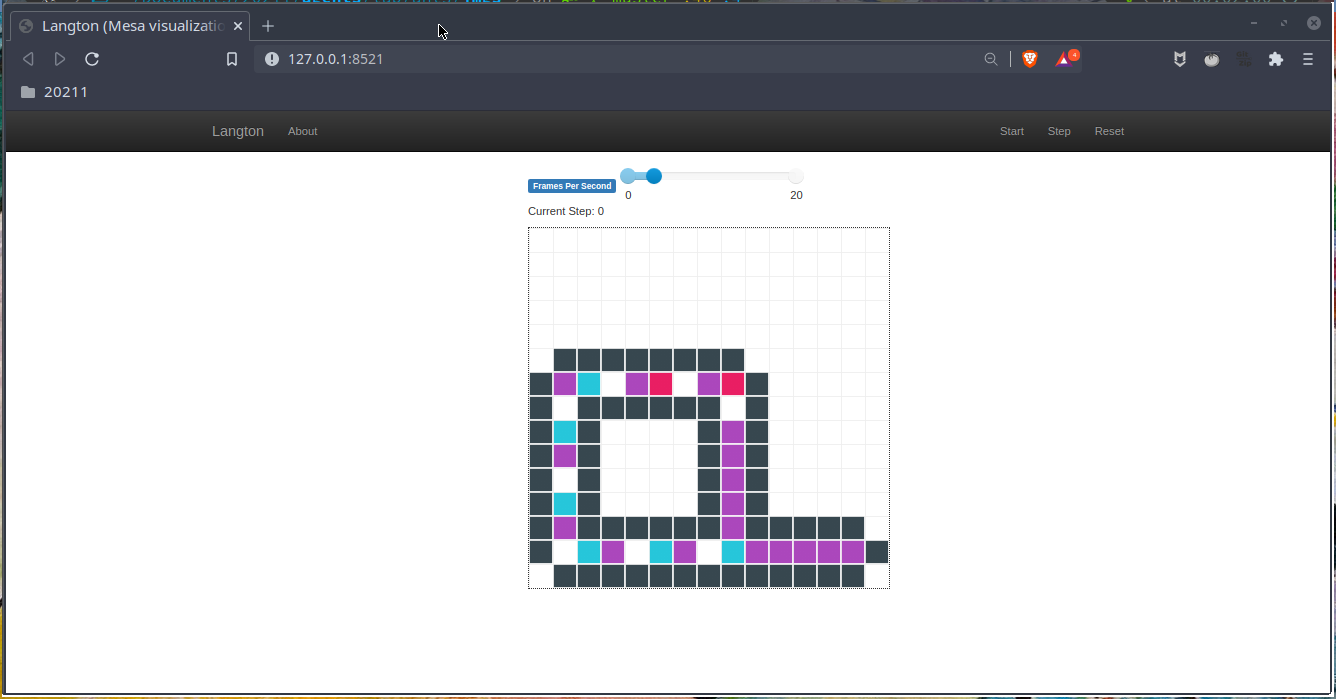
\includegraphics[width=\textwidth]{imgs/lang_ui.png}
  \caption{Visualización del loop de Langton}
  \label{fig:langton-ui}
\end{figure}

La implementación se realizó en \textit{mesa}. La interfaz gráfica resultante se
puede ver en la figura \ref{fig:langton-ui}. El tamaño de la malla se alteró
para los diferentes ejercicios, con el fin de tener una buena visualización.

\subsubsection{Segunda generación}

Muestre como se ve el sistema en el tiempo 151. Este corresponde al fin de la
formación de la segunda generación de loops.

La visualización del sistema se puede ver en \ref{fig:langton-150}. Se pueden
ver dos loops idénticos perfectamente formados, con la diferencia de que el loop
original está rotado.

\begin{figure}
  \centering
  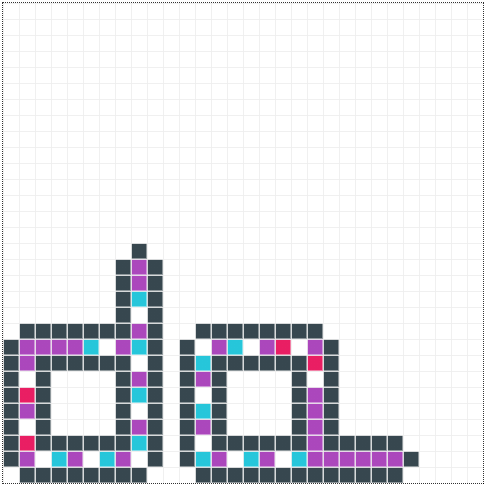
\includegraphics[width=0.5\textwidth]{imgs/lang2.png}
  \caption{Loop de Lagton al tiempo 150}
  \label{fig:langton-150}
\end{figure}

\subsubsection{Séptima generación}

Muestre como se ve el sistema en la generación 7. ¿Cuántos loops activos,
muertos y moribundos hay?

\begin{figure}
  \centering
  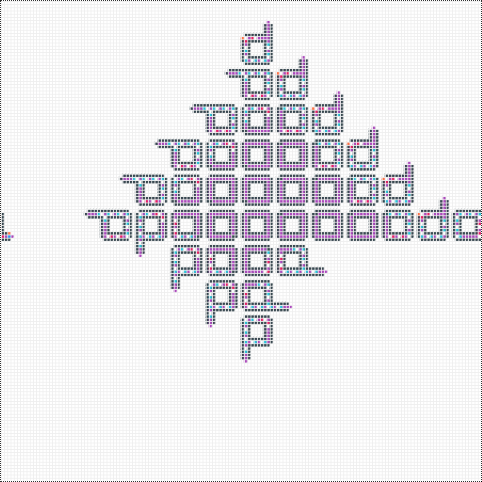
\includegraphics[width=0.5\textwidth]{imgs/lang_gen7.png}
  \caption{Loop de Lagton después de siete generaciones}
  \label{fig:langton-7}
\end{figure}

La visualización del sistema se puede ver en la figura \ref{fig:langton-7}.
Tiene un total de 11 loops muertos, que tiene un núcleo sin flujo de
información. Tiene 10 loops moribundos, que aún tiene flujo de información pero
no canales nuevos a donde mandarla. Y tiene 18 loops activos, que tiene flujo y
canales activos. En total hay 39 loops en esta generación.

\subsubsection{Crecimiento}

Deduzca una fórmula para el crecimiento de la colonia de loops.

\begin{table}
  \centering
  \begin{tabular}{| c | c | c | c | c |}
    \hline
    Gen & Vivo & Moribundo & Muerto & Total\\
    \hline
    1 & 1 & 0 & 0 & 1\\
    2 & 2 & 0 & 0 & 2\\
    3 & 4 & 0 & 0 & 4\\
    4 & 7 & 1 & 0 & 8\\
    5 & 10 & 4 & 1 & 15\\
    6 & 14 & 6 & 5 & 25\\
    7 & 18 & 10 & 11 & 39\\
    8 & 22 & 14 & 21 & 57\\
    \hline
  \end{tabular}
  \caption{Evolución de la colonia de loops}
  \label{tab:langton-evol}
\end{table}

\begin{table}
  \centering
  \begin{tabular}{| c | c | c | c | c |}
    \hline
    Gen & Génesis & Primogénito & Otro & Total\\
    \hline
    1 & 1 & 0 & 0 & 1\\
    2 & 1 & 1 & 0 & 2\\
    3 & 1 & 3 & 0 & 4\\
    4 & 1 & 5 & 1 & 7\\
    5 & 0 & 7 & 3 & 10\\
    6 & 0 & 8 & 6 & 14\\
    7 & 0 & 8 & 10 & 18\\
    8 & 0 & 8 & 14 & 22\\
    \hline
  \end{tabular}
  \caption{Evolución de los tipos de loop vivos}
  \label{tab:langton-alive}
\end{table}

Para tener una referencia, en las tablas \ref{tab:langton-evol} y
\ref{tab:langton-alive} están los resultados de simular y contar directamente
como crece la colonia de loops.

En cada generación, cada loop vivo se replica, así que la cantidad total de
loops se podría ver como

\begin{equation*}
  \eta(t) = \begin{cases}
    1, \text{ si }t = 1 \\
    \eta(t-1) + \alpha(t-1) \text{ en otro caso }
  \end{cases}
\end{equation*}

Y expandiendo la fórmula, se puede reescribir como

\begin{equation}
\label{eq:langton-n}
  \eta(t) = 1 + \sum_{k = 1}^{t-1}{\alpha(k)}
\end{equation}

donde $\alpha(t)$ es la cantidad de ciclos vivos durante el tiempo $t$.

Para encontrar $\alpha(t)$ hay que analizar la dinámicas de los loops.

Cada loop tiene un comportamiento bien definido. En cada paso, intentaran crear
otro loop en la dirección dada por su tentáculo. En caso de no poder, el
tentáculo se retracta y el loop empieza a morir. En caso de sí poder, se crea el
nuevo loop, se gira en sentido antihorario y se vuelve a intentar.

Pero, aunque todos los ciclos tienen el mismo comportamiento, reaccionan
diferente dependiendo de los obstáculos que se encuetren. Hay tres escenarios
para un loop.

\begin{itemize}
  \item Génesis

    El loop inicial. Como no tiene obstáculos, tiene cuatros descendientes antes
    de morir.

  \item Primogénito

    Son los primogénitos de los cuatros descendientes del loop inicial. Al ser
    creados, estos crean un nuevo primogénitos siguiendo la dirección en la que
    fueron creados. Al siguiente turno, rotan y crean otro loop 90 grados en
    sentido antihorario. En el siguiente turno, vuelven a rotar, se topan con su
    padre y mueren

    Así que tienen dos descendientes.

  \item Otro

    Corresponden a los segundo hijos de los primogénitos. Estos crecen de forma
    perpendicular a las direcciones de los primogénitos. Al crearse, crean otro
    loop en la misma dirección en la que fueron credos. Luego rotan, se
    encuentran con otro loop y mueren. Estos tienen un descendiente.

\end{itemize}

El loop inicial tarda en crear sus descendientes, así que las cuatro primeras
generaciones se pueden pensar como un periodo de estabilización. Además, cada
uno de sus descendientes debe completar un ciclo suyo para terminar de
estabilizar la dinámica. Como el último descendiente del loop inicial es creado
en la generación $4$, entonces en la generación $6$ se podría decir que la
dinámica global del sistema se estabiliza.

En este punto, no hay loop iniciales. Hay cuatro primogénitos en su primera fase
y cuatro en su segunda fase, dando un total de ocho. Para los
otros loops, cada uno se replicó y murió, asi que se mantiene esa cantidad, pero
además cada primogénito en segunda fase crea uno nuevo. Hay entonces
$\omega(t) = \omega(6) + 4(t-6), t \ge 6$ otros loops.

Así que para $t \ge 6$ se tiene que

\begin{equation*}
  \alpha(t) = 8 + \omega(t) = 8 + \omega(6) + 4(t-6) = 4t + \omega(6) - 16
\end{equation*}

De la tabla \ref{tab:langton-alive} se tiene que $\omega(6) = 6$, así que la
fórmula queda como

\begin{equation}
\label{eq:langton-a}
  \alpha(t) = 4t - 10
\end{equation}

Entonces, restrigiendo que $t > 6$, la ecuación \ref{eq:langton-n} se puede
reescribir como

\begin{align*}
  \eta(t) &= \eta(6) + \sum_{k = 6}^{t-1}{(4k - 10)}\\
  &= \eta(6) + 4 (\sum_{k=6}^{t-1}{k}) - 10(t-6)\\
  &= \eta(6) + 4 (\sum_{k=6}^{t-1}{k}) - 10t + 60\\
\end{align*}

Y de la tabla \ref{tab:langton-evol} se puede obtener que que $\eta(6) = 25$.
Por lo que

\begin{align*}
  &= 25 + 4 (\sum_{k=6}^{t-1}{t}) - 10t + 60\\
  &= 4 (\frac{t(t-1)}{2} - \frac{6(7)}{2}) - 10t + 85\\
  &= 2t(t-1) - 60 - 10t + 85 \\
  &= 2t^{2} - 12t + 25\\
\end{align*}

Así que para $t > 6$, la cantidad de loops en la colonia en la generación $t$
está dada por

\begin{equation}
\label{eq:langton-final}
  \eta(t) = 2t^{2} - 12t + 25
\end{equation}

En la tabla \ref{tab:langton-evol} se puede ver que la fórmula funciona para
$t = 7, 8$.

\section{Proyeto final}

Marco Dorigo propuso un modelo basado en el comportamiento social de las
hormigas para optimización sobre gráficas \cite{Dorigo_1996}. Este intenta
imitar los rastros de feromonas usados por las hormigas para comunicar donde se
encuentran las mejores fuentes de comida. Esta técnica fue utilizada con éxito
para aproximar soluciones a problemas $NP$-Duros, como el problema del agente
viajero, TSP.

Debido a su eficacia, muchas variantes han surgido \cite{Dorigo_2006}. Para
proyecto final, se propone primero implementar una visualización de alguna de
las variantes del modelo para resolver el problema de TSP. Luego, como extensión
del modelo, adaptar algún otro problema $NP$-Completo para ser resuelto por el
modelo de colonia de hormigas. Esto aún está al aire, pero una propuesta
interesante sería resolver un cubo de Rubik \cite{Demaine_2018}, que
recientemente se demostró $NP$-Completo.

\printbibliography

\end{document}